\chapter{Results}
This chapter presents all the experiment results for each experiment and evaluation, aimed at addressing the research questions.
The result are divided into four sections, including pre-training, image-text matching, visual question answering, and the evaluation result of varying the POS masking percentage.

\section{Pre-training}
To address the question of how masking each \acrshort{pos} affects the performance and training loss of \acrshort{vl} pre-training models, we present all relevant results in this section.  
All losses, including \acrshort{mlm}, \acrshort{itc}, and \acrshort{itm}, along with the Flickr30K evaluation results, are provided.  
The loss values are plotted on a logarithmic scale to visualize improvements over time across different POS masking strategies.  
The results from training the ALBEF model using the same dataset are also included for consistent comparison.
We also provided the histrogram of each part-of-speech tag in the pre-training dataset as shown in Figure~\ref{fig:pos_count}.

\subsection{Flickr30K}
The Flickr30K evaluation results are shown in Table \ref{tab:flickr30k}, which presents the top-1, top-5, and top-10 retrieval scores for both \acrshort{tr} and \acrshort{ir} tasks across different training methodologies.  
By comparing r@1 performance for both \acrshort{tr}, and \acrshort{ir}, the model with determiner masking achieves the highest overall performance.
Among the non-functional group, masking NOUN yields the best performance.
By masking ADV and PROPN causes the most significant degradation compared to the random masking baseline.

\begin{table}[h]
    \centering
    \caption{Flickr30K benchmark image retrieval result.}
    \label{tab:flickr30k}
    \begin{adjustbox}{width=0.8\textwidth}
        \begin{tabular}{ll|ccc|ccc}
            \hline
            \multicolumn{2}{c|}{\multirow{3}{*}{\textbf{Masking Method}}} & \multicolumn{6}{c}{\textbf{Flickr30K}} \\
            \multicolumn{2}{l|}{} & \multicolumn{3}{c|}{\acrshort{tr}} & \multicolumn{3}{c}{\acrshort{ir}} \\
            \multicolumn{2}{l|}{} & r@1 & r@5 & r@10 & r@1 & r@5 & r@10 \\
            \hline
            \multicolumn{2}{l|}{ALBEF} & 70.40 & 89.50 & 94.00 & 54.66 & 82.02 & 88.70 \\
            \hline
            \multicolumn{2}{l|}{Random Masking} & 67.00 & 88.00 & 93.75 & 52.61 & 80.14 & 87.76 \\
            \hline
            \multirow{5}{*}{Non-functional} & NOUN & 67.15 & 88.60 & 94.65 & 52.73 & 80.45 & 87.79 \\
            & VERB & 54.85 & 82.85 & 90.05 & 43.82 & 73.84 & 82.82 \\
            & ADJ & 62.30 & 87.30 & 92.40 & 47.39 & 75.47 & 84.06 \\
            & ADV & 46.85 & 76.25 & 85.75 & 36.40 & 66.38 & 76.78 \\
            & PROPN & 44.85 & 74.40 & 84.10 & 34.91 & 64.09 & 75.01 \\
            \hline
            \rowcolor{gray} \multirow{4}{*}{Functional} & DET & 71.05 & 92.00 & 95.30 & 56.01 & 81.93 & 88.59 \\
            & AUX  & 52.10 & 79.60 & 88.20 & 41.13 & 70.92 & 80.68 \\
            & PRON & 51.45 & 78.80 & 87.10 & 39.97 & 69.58 & 79.32 \\
            & ADP & 65.05 & 88.25 & 93.40 & 51.19 & 78.83 & 85.15 \\
            \hline
        \end{tabular}
    \end{adjustbox}
\end{table}

From the training loss curves, it is evident that different POS categories affect the convergence behavior in difference ways.
The loss for \acrshort{mlm}, \acrshort{itc}, and \acrshort{itm} are displayed in the Figure \ref{fig:mlm_loss_pretrain}, Figure \ref{fig:itc_loss_pretrain}, and Figure \ref{fig:itm_loss_pretrain} respectively
For both \acrshort{itm} and \acrshort{itc}, the loss curves are similar in behavior and follow a consistent order relative to each other.
In the \acrshort{mlm} loss graph, we can see that \acrshort{pos} masking in the functional group result in lower loss, while those in the non-functional group show higher loss, and the random masking show the highest loss by the end of training.

Taken together, the results show that masking each POS impacts both the training loss trajectory and final model performance in distinct ways.  
By observing the \acrshort{mlm} loss graph, we find that non-functional \acrshort{pos} are more difficult for the model to learn through the \acrshort{mlm} task, whereas functional \acrshort{pos} are learned more quickly.
The ranking of the performance for each \acrshort{pos} masking method aligns with the \acrshort{itm} and \acrshort{itc} loss curves, where a lower loss corresponds to higher retrieval accuracy.

\begin{figure}[H]
    \caption{\acrshort{mlm} loss curves for different \acrshort{pos} masking strategies (log scale).}
    \label{fig:mlm_loss_pretrain}
    \centering
    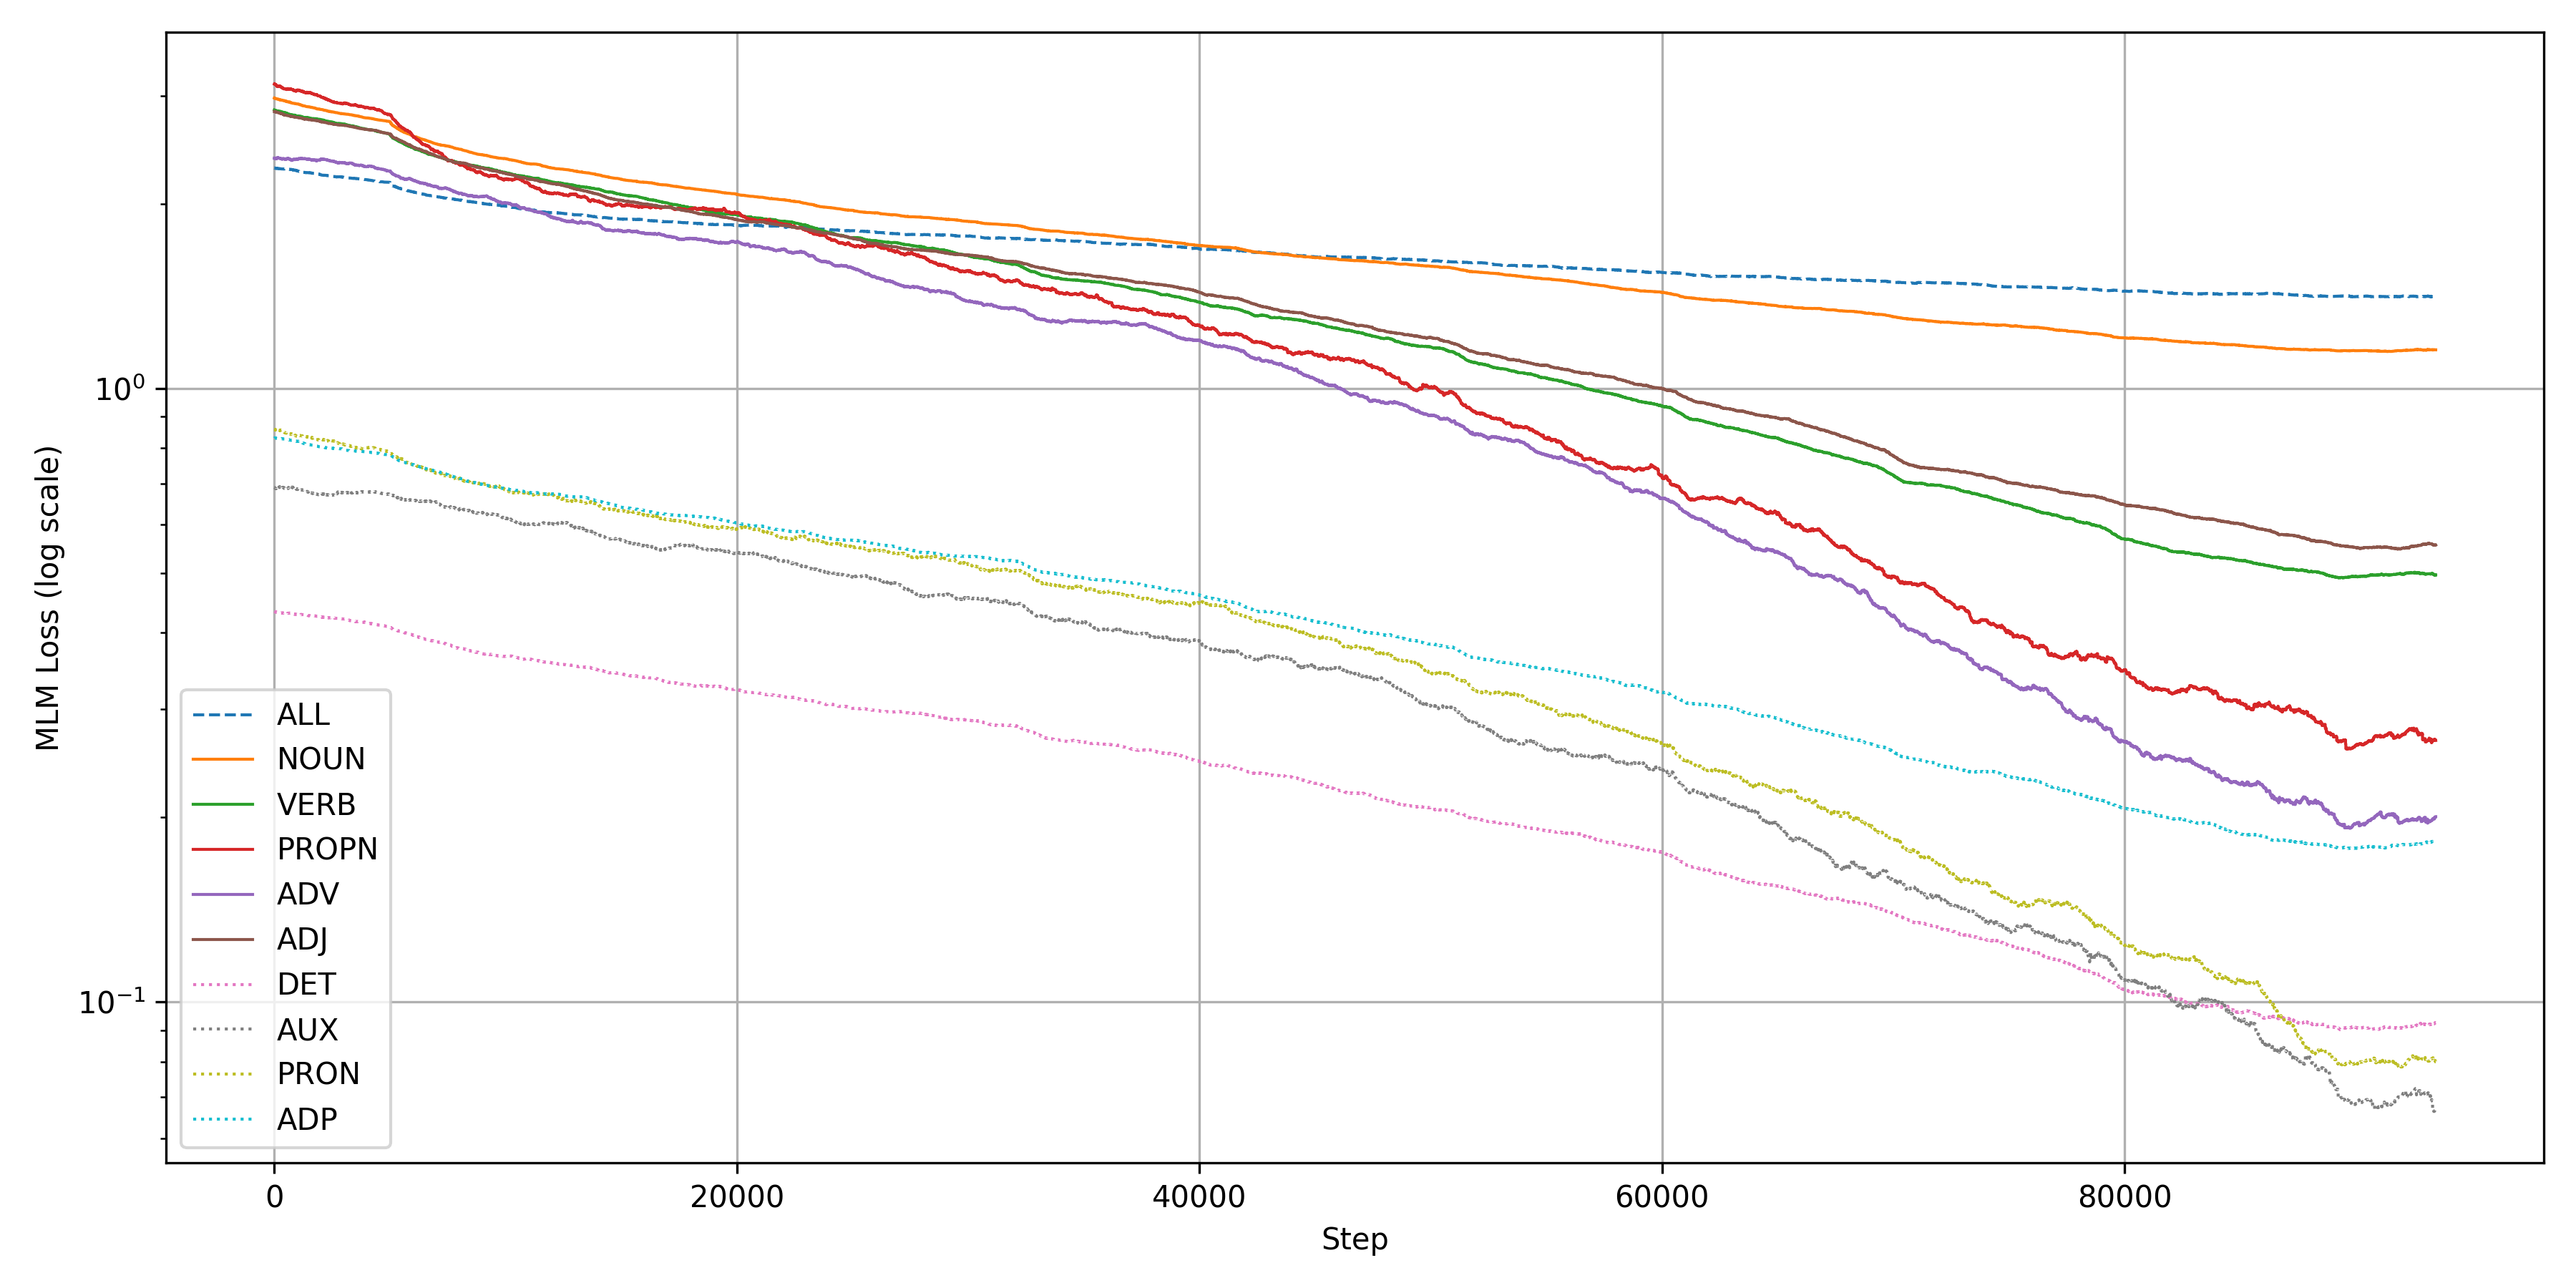
\includegraphics[width=\textwidth]{Images/graph/mlm.png}
\end{figure}

\begin{figure}[H]
    \caption{\acrshort{itc} loss curves for different \acrshort{pos} masking strategies (log scale).}
    \label{fig:itc_loss_pretrain}
    \centering
    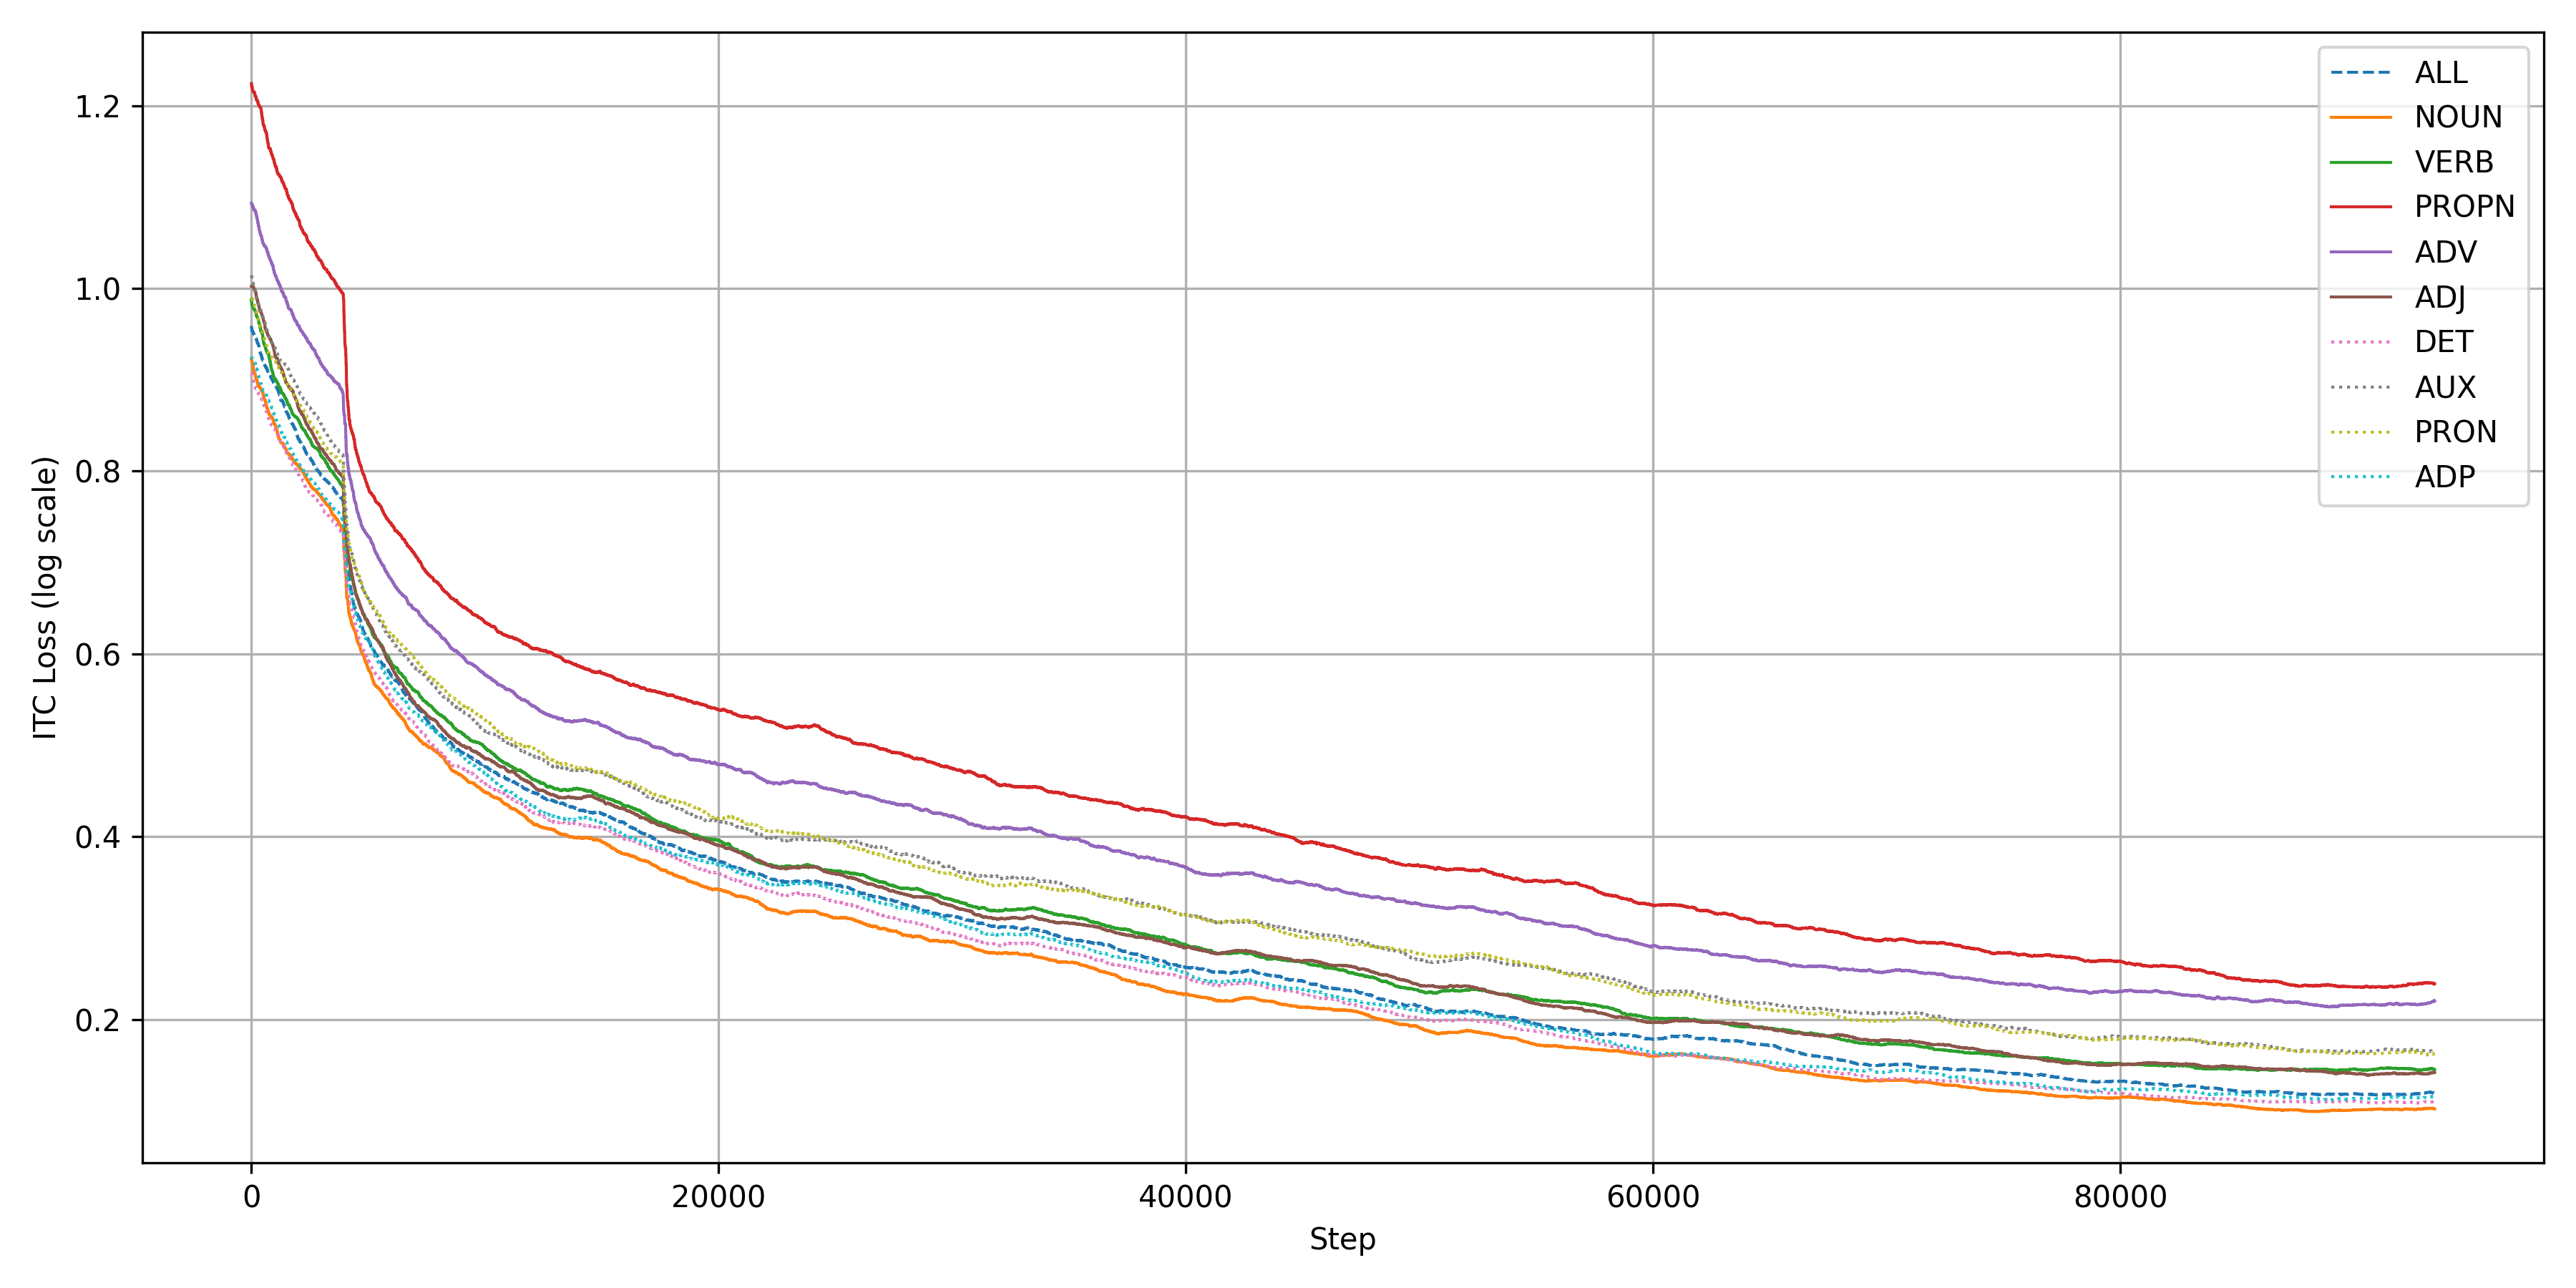
\includegraphics[width=\textwidth]{Images/graph/itc.png}
\end{figure}

\begin{figure}[H]
    \caption{\acrshort{itm} loss curves for different \acrshort{pos} masking strategies (log scale).}
    \label{fig:itm_loss_pretrain}
    \centering
    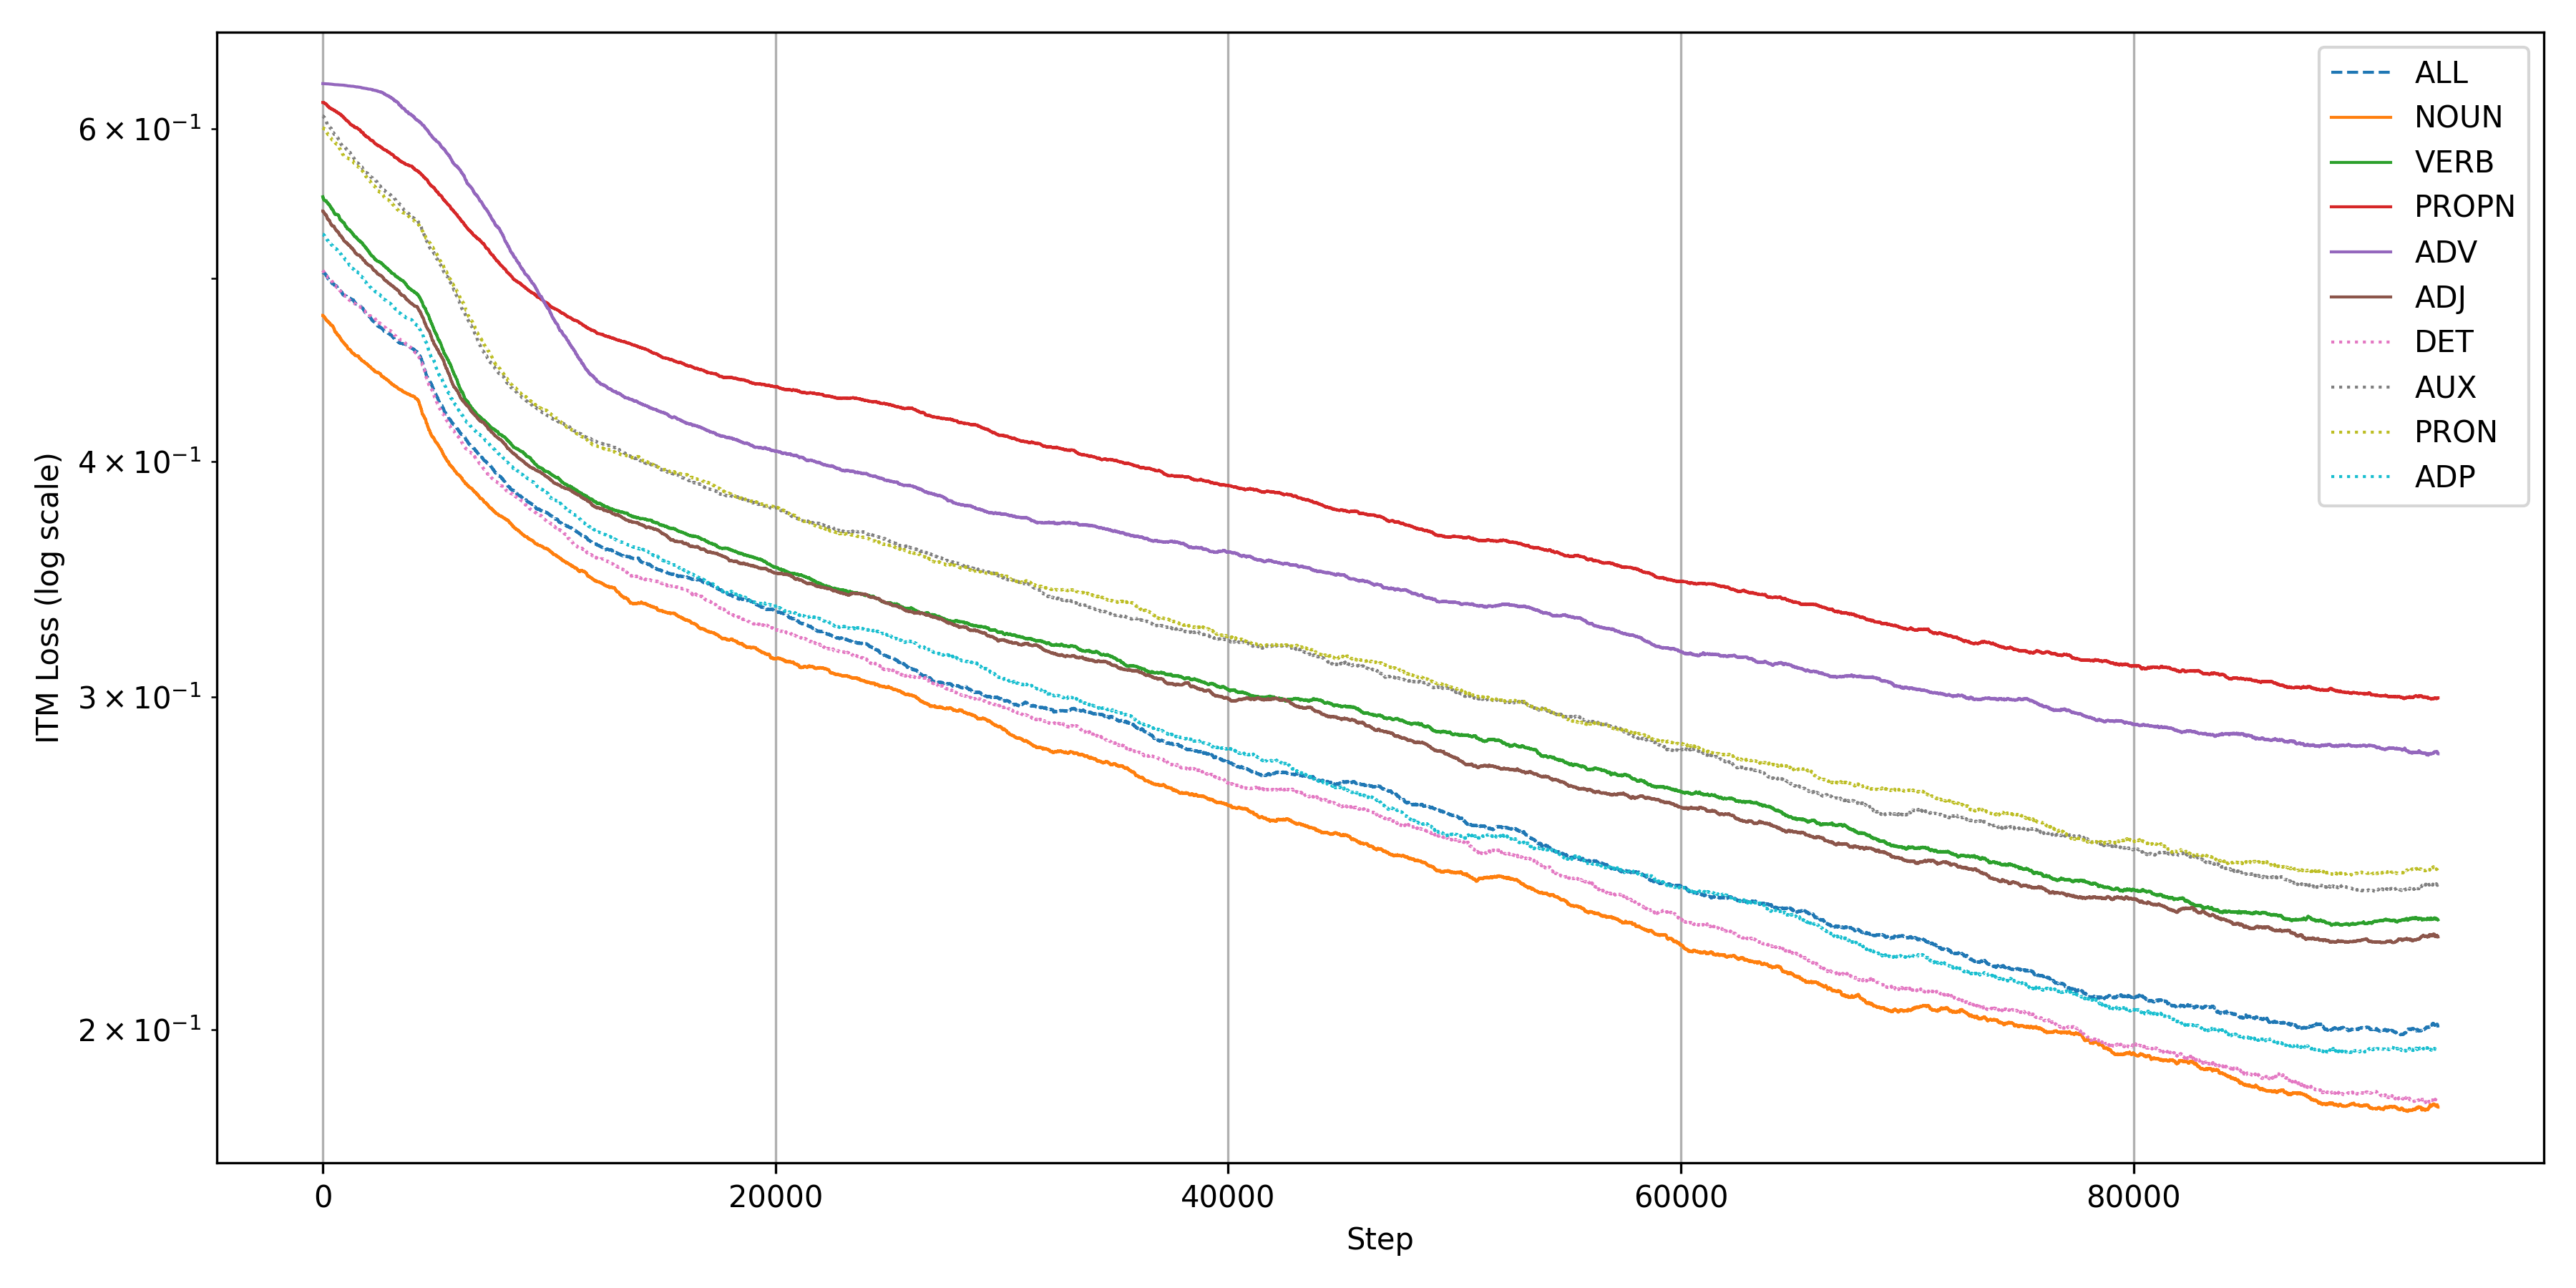
\includegraphics[width=\textwidth]{Images/graph/itm.png}
\end{figure}

% \begin{figure}[h]
%     \caption{\acrshort{mlm} loss curves for different \acrshort{pos} masking strategies (log scale).}
%     \label{fig:mlm_loss_pretrain}
%     \begin{center}
%         \begin{adjustbox}{width=0.8\textwidth}
%             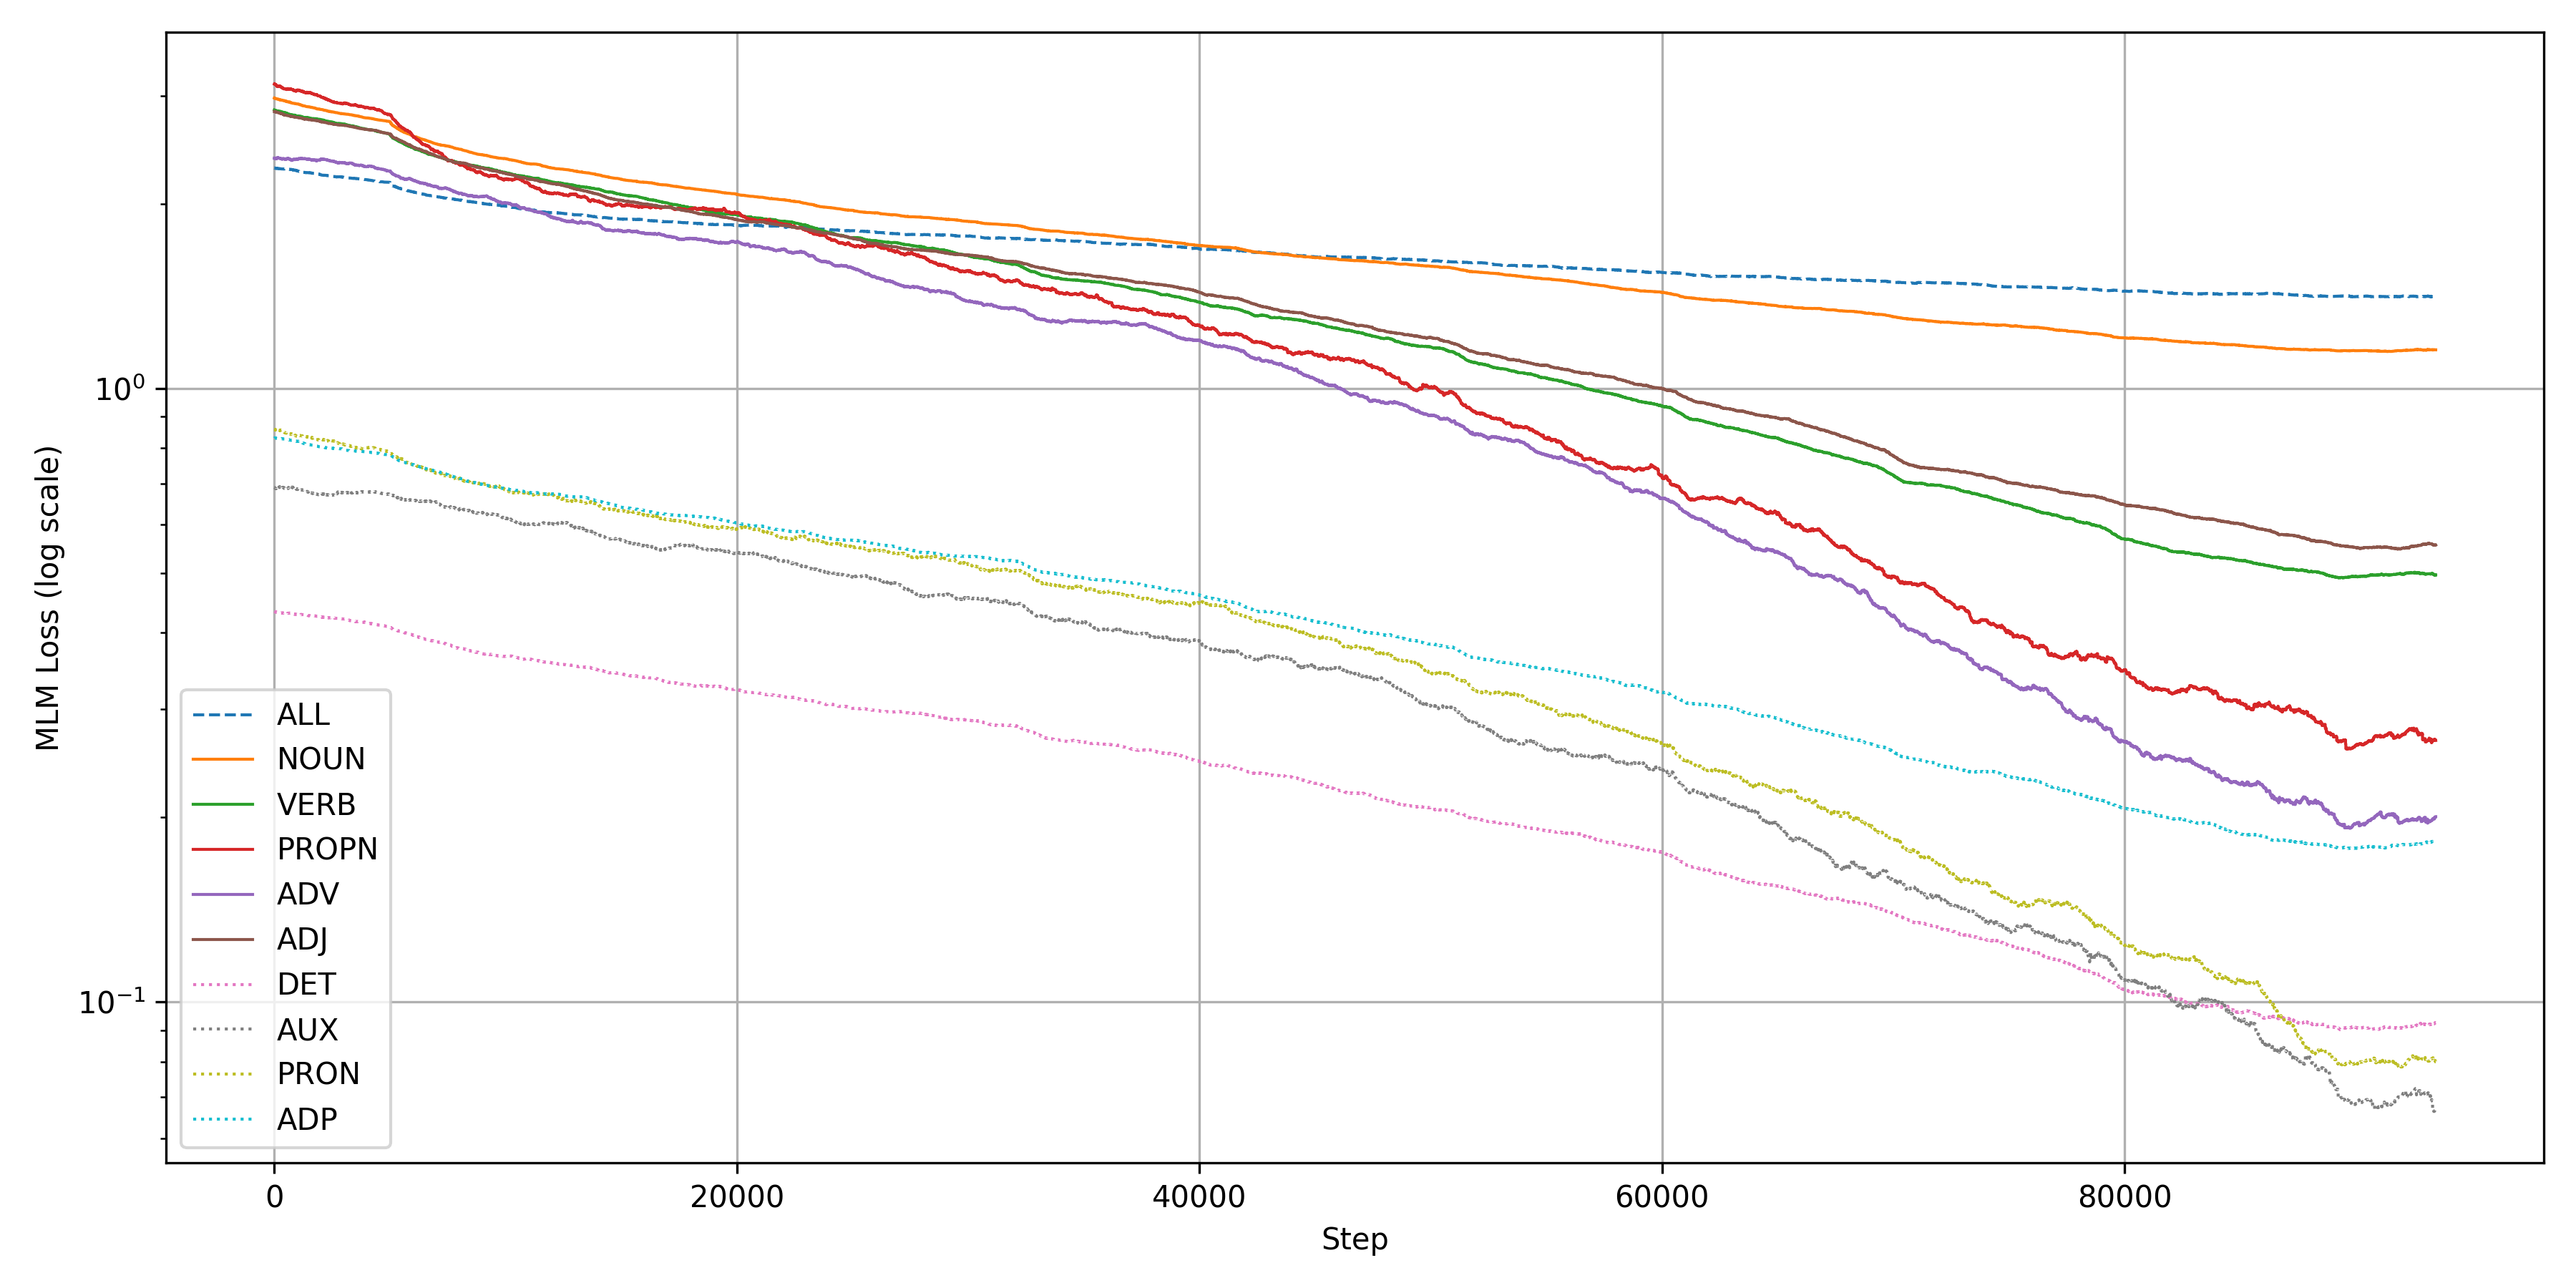
\includegraphics[width=1\textwidth]{Images/graph/mlm.png}
%         \end{adjustbox}
%     \end{center}
% \end{figure}

% \begin{figure}[h]
%     \caption{\acrshort{itc} loss curves for different \acrshort{pos} masking strategies (log scale).}
%     \label{fig:itc_loss_pretrain}
%     \begin{center}
%         \begin{adjustbox}{width=0.8\textwidth}
%             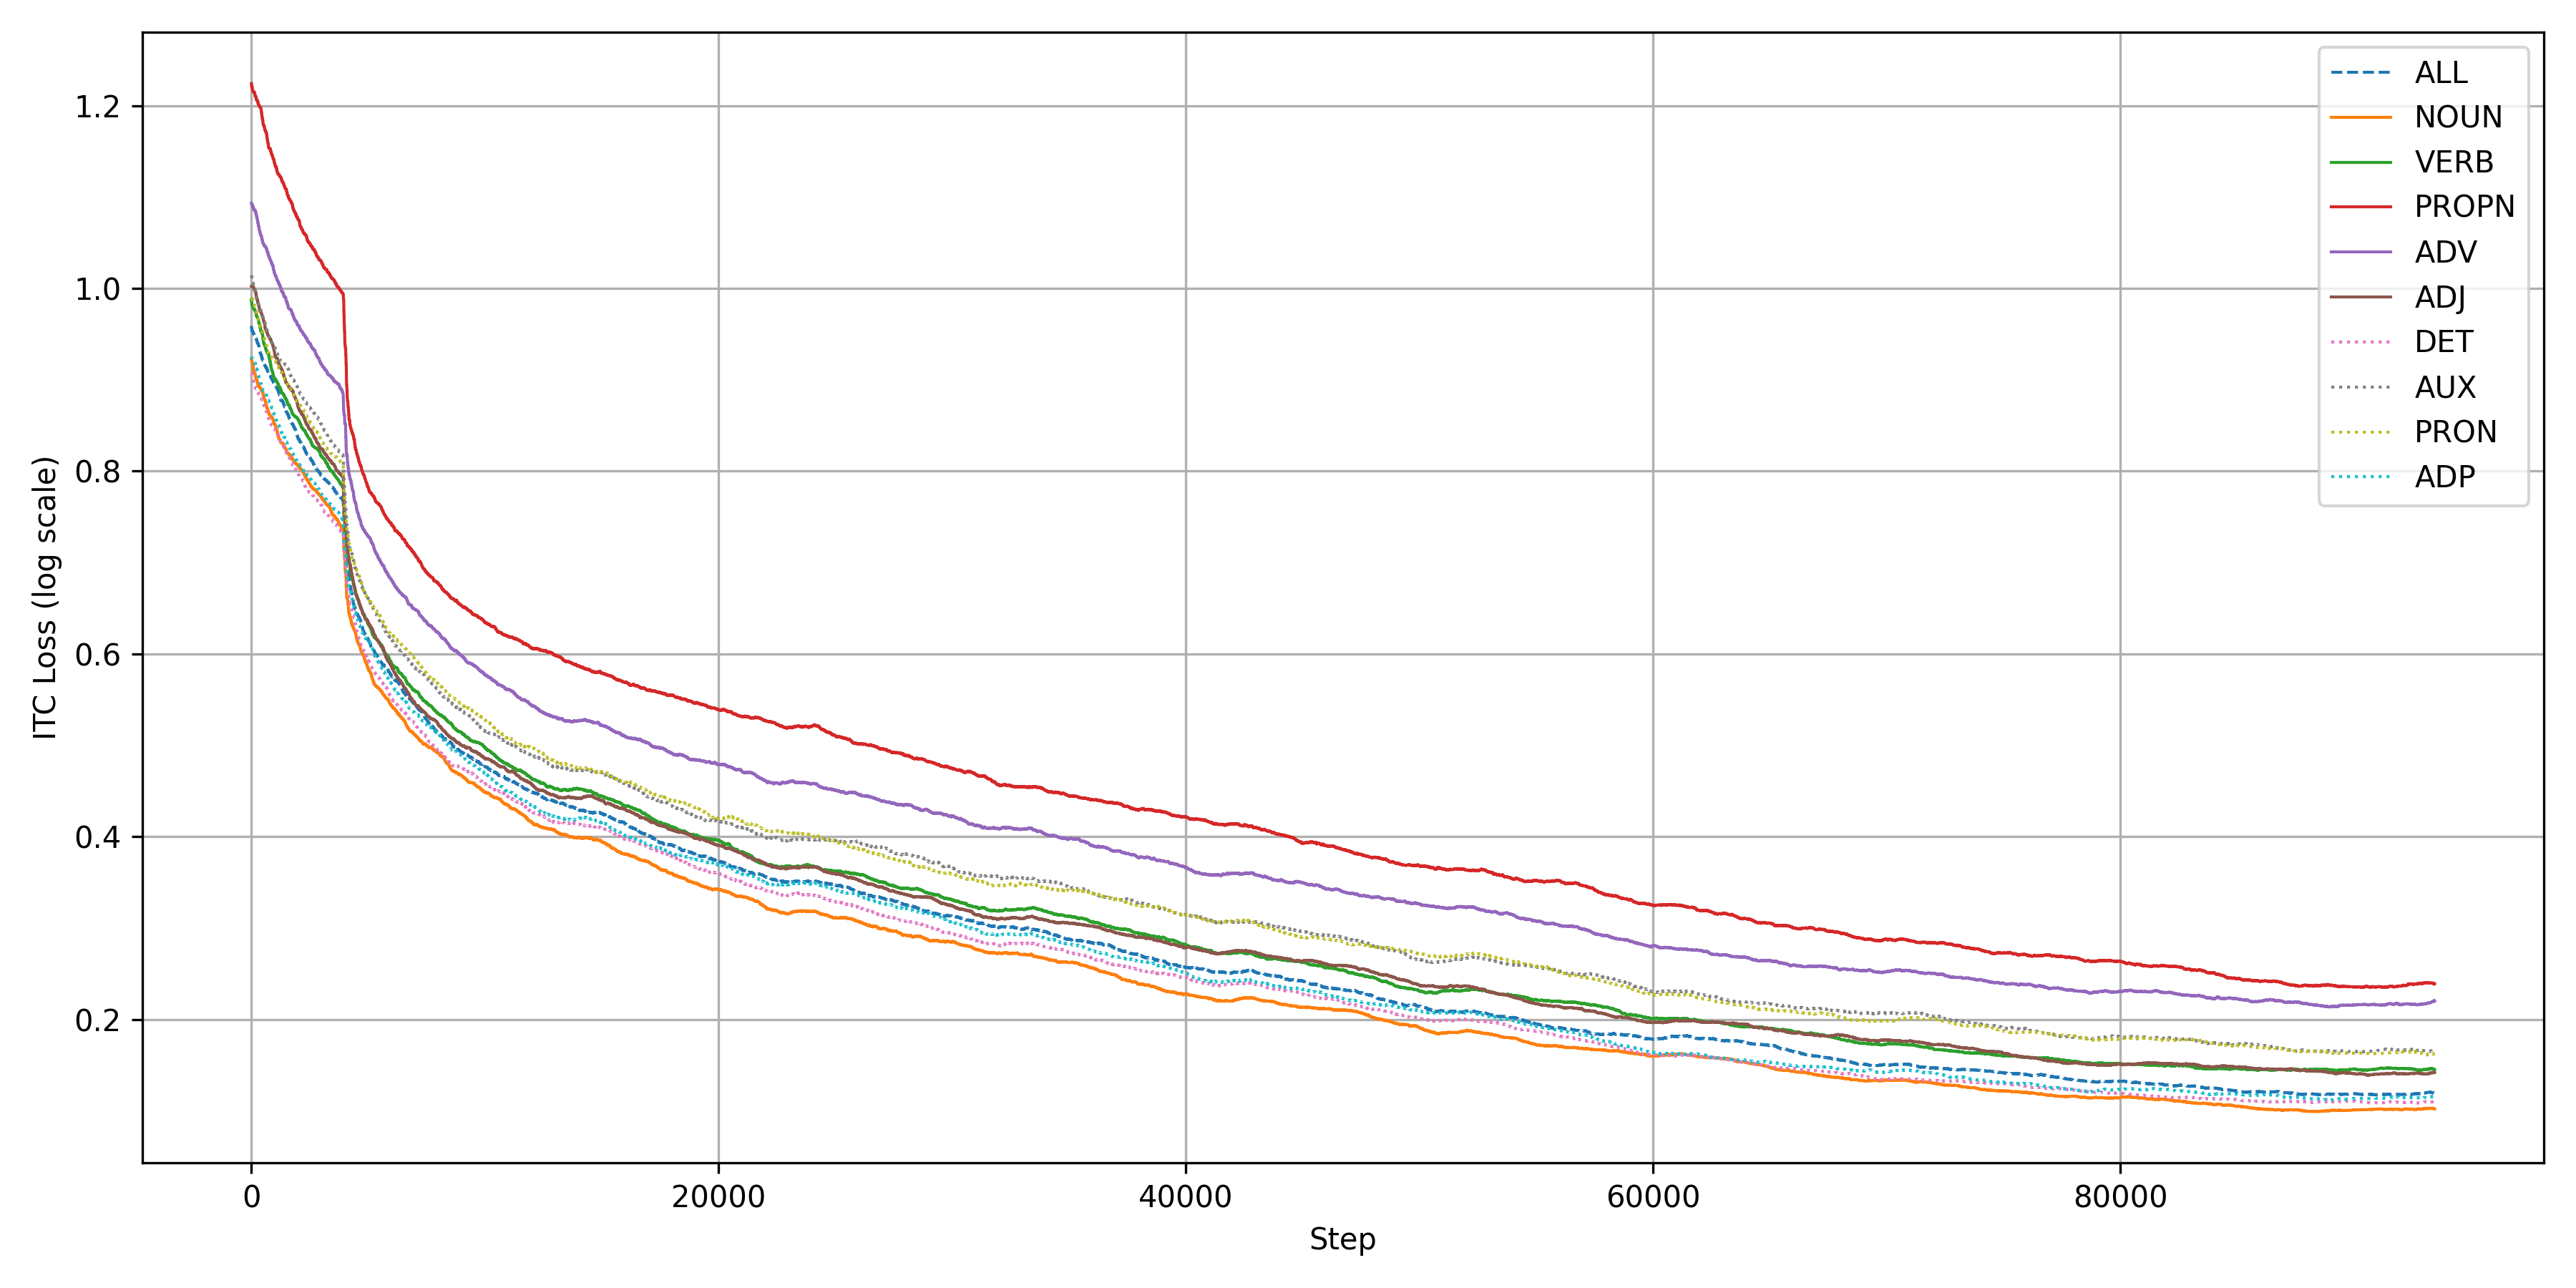
\includegraphics[width=1\textwidth]{Images/graph/itc.png}
%         \end{adjustbox}
%     \end{center}
% \end{figure}

% \begin{figure}[h]
%     \caption{\acrshort{itm} loss curves for different \acrshort{pos} masking strategies (log scale).}
%     \label{fig:itm_loss_pretrain}
%     \begin{center}
%         \begin{adjustbox}{width=0.8\textwidth}
%             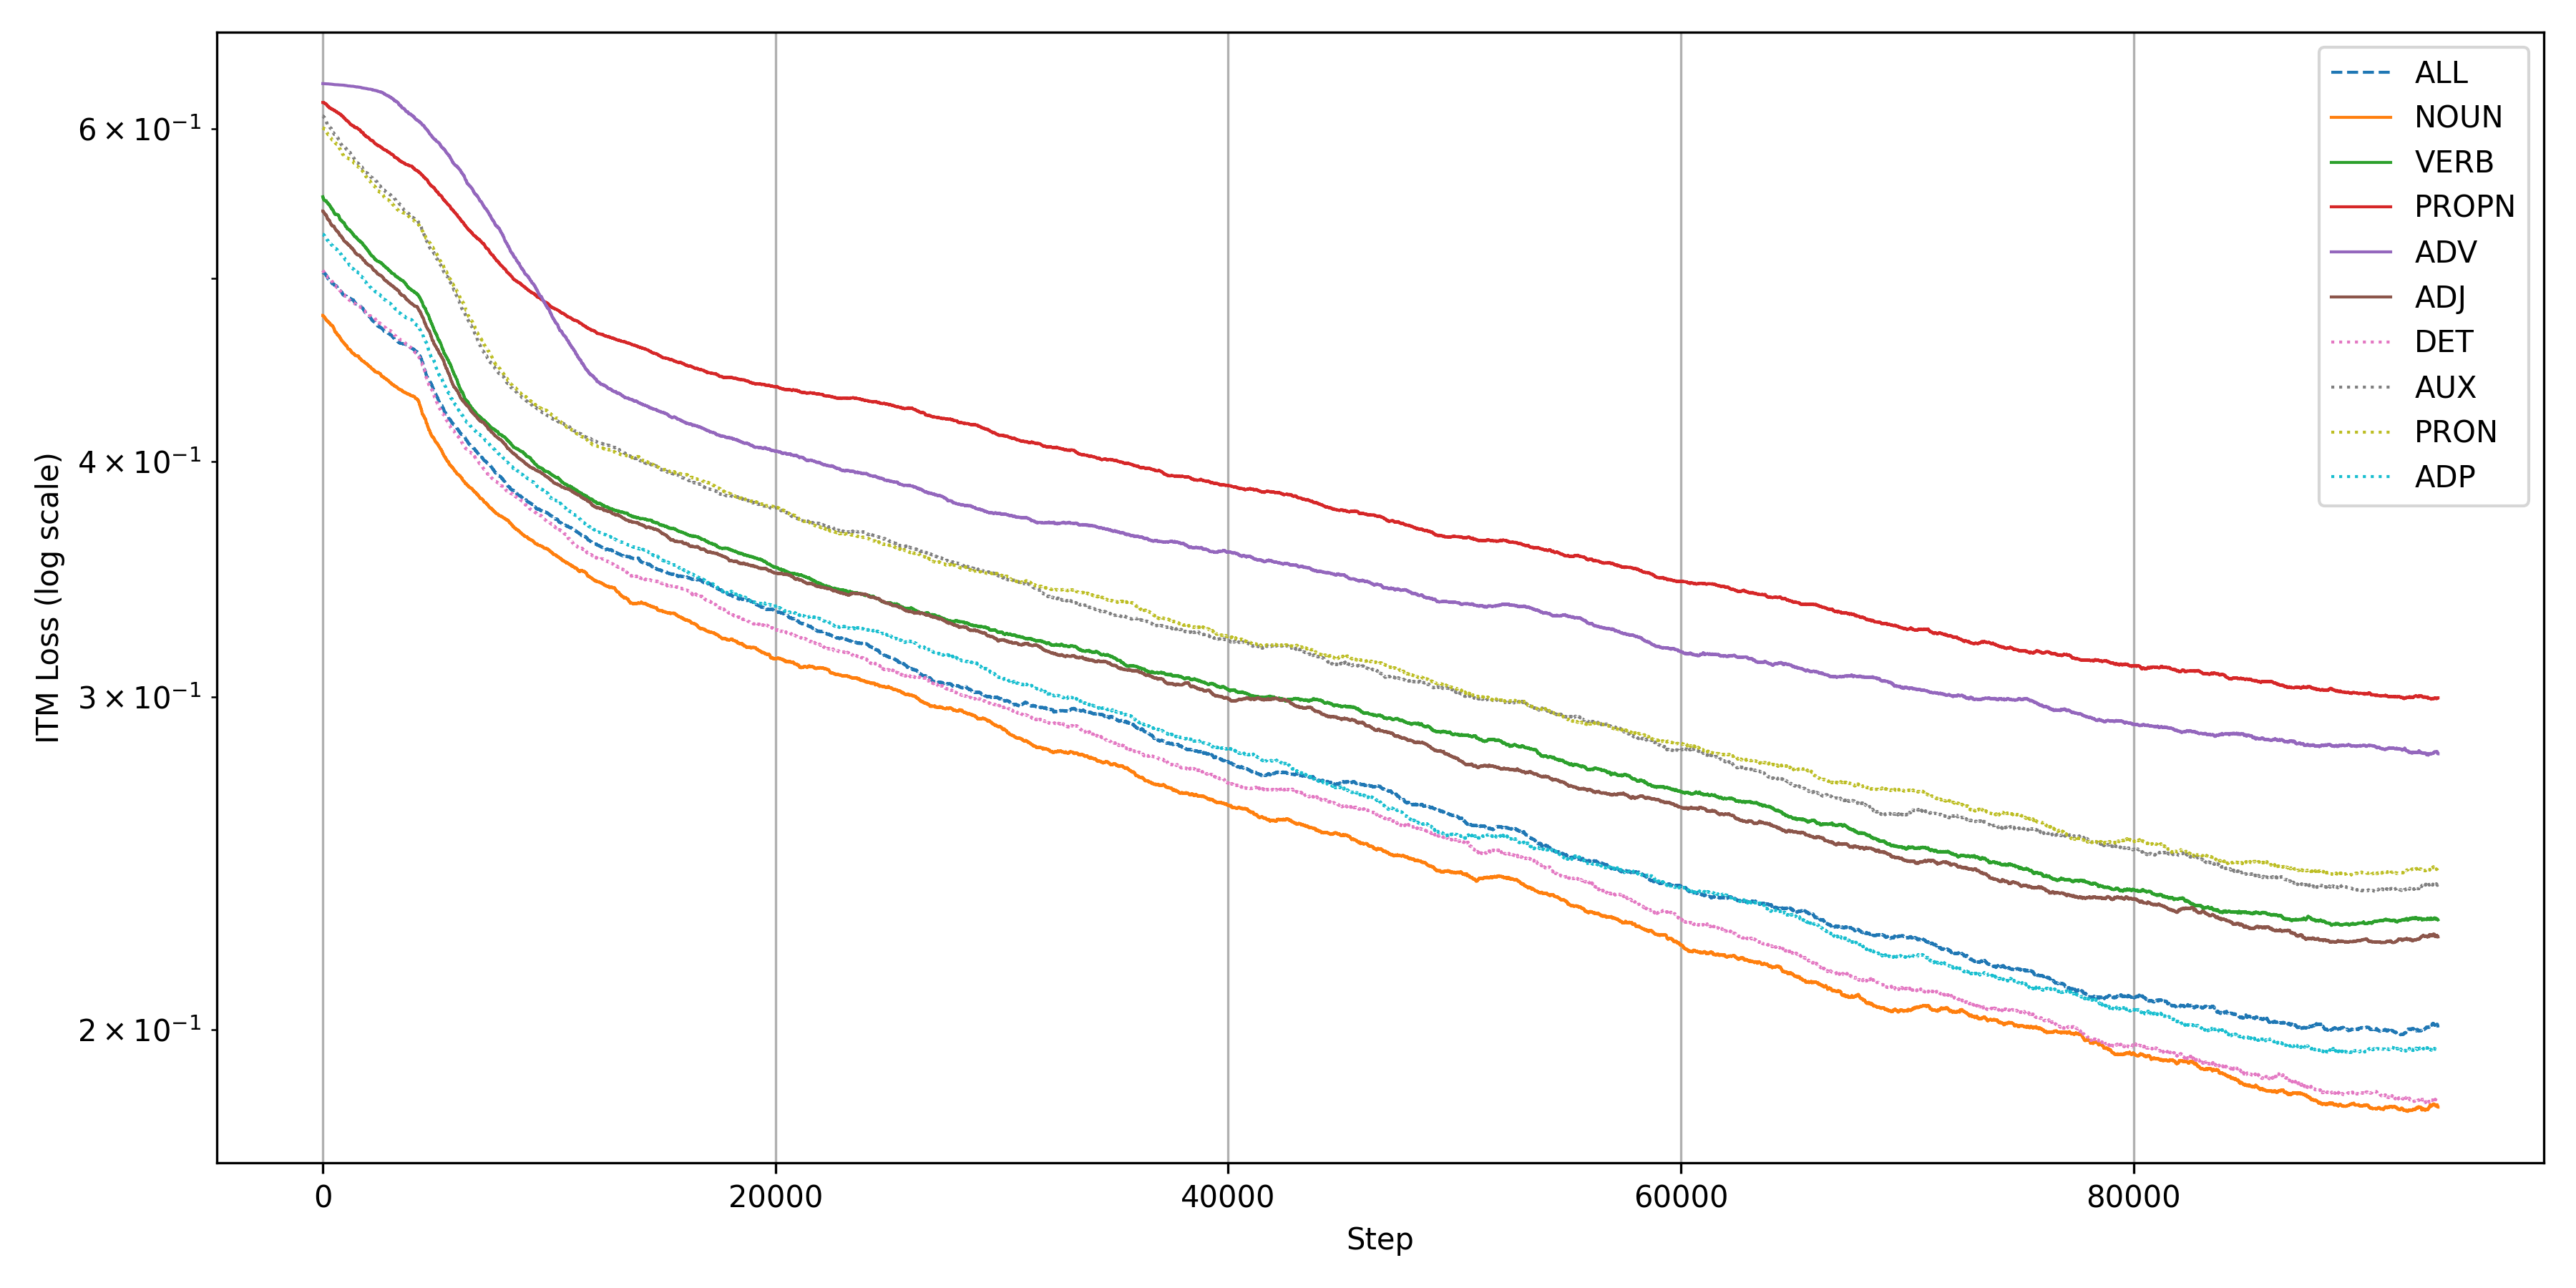
\includegraphics[width=1\textwidth]{Images/graph/itm.png}
%         \end{adjustbox}
%     \end{center}
% \end{figure}

\subsection{Histogram of POS tag}
This section provides a visualization of tokens categorized by their \acrshort{pos} from the training dataset, as shown in Figure \ref{fig:pos_count}.
The histogram illustrates the frequency distribution of \acrshort{pos} tags, sorted from the most to least common.
NOUN tokens dominate the dataset, followed by ADP, DET, VERB, and ADJ, while categories such as SYM, INTJ, X, PUNCT, and SPACE appear rarely in the training dataset.

\begin{figure}[H]
    \caption{Histogram of POS tag frequencies in the training dataset (sorted by frequency).}
    \label{fig:pos_count}
    \centering
    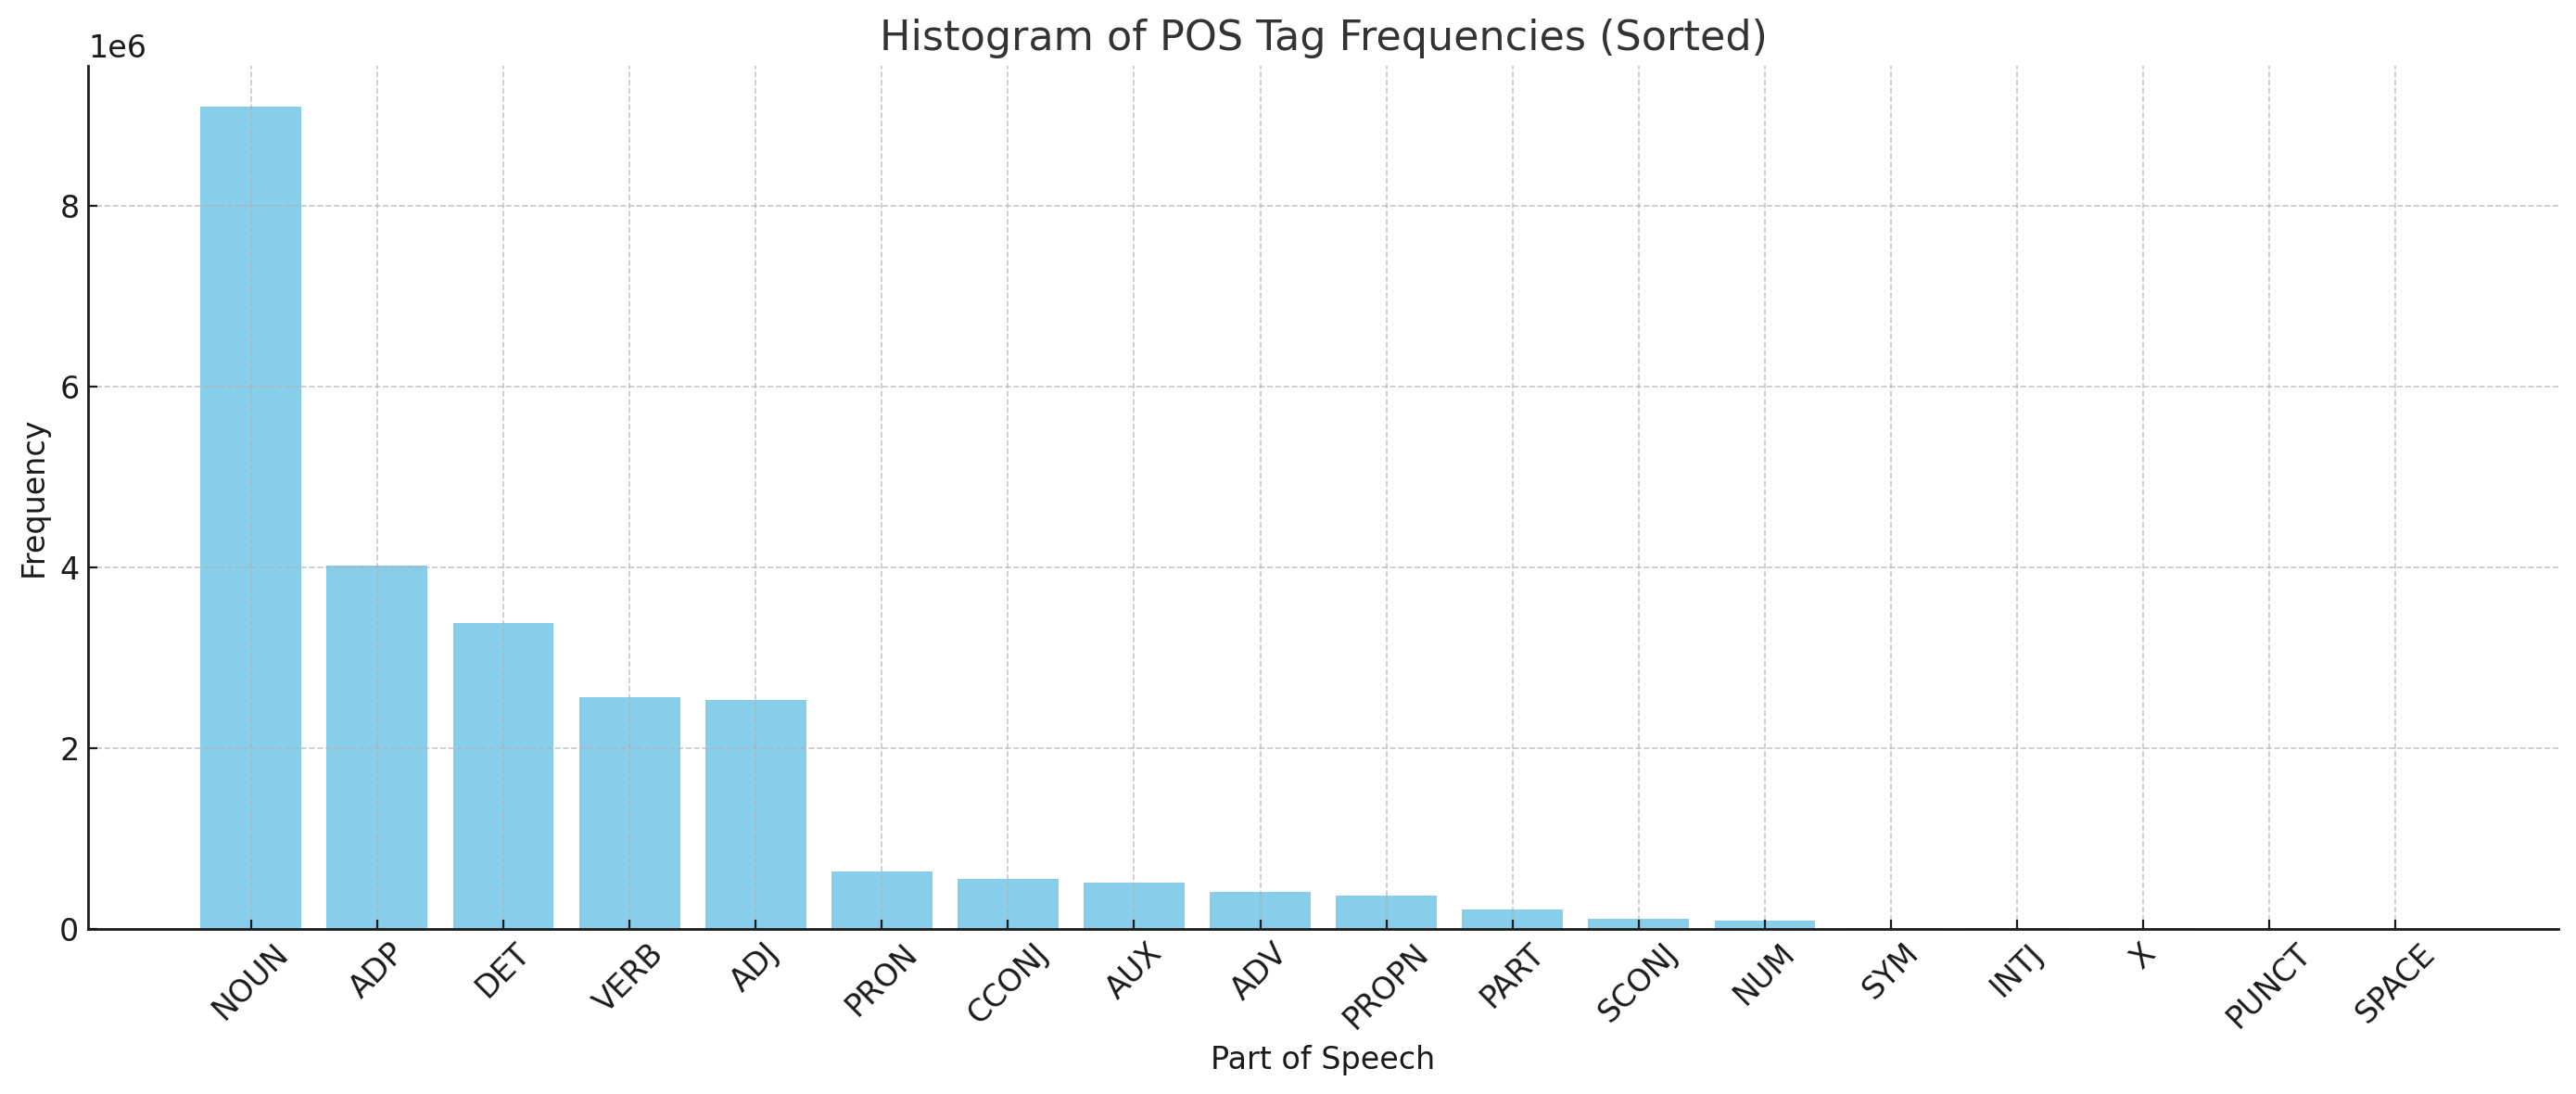
\includegraphics[width=0.8\textwidth]{Images/graph/pos_count.png}
\end{figure}

\section{Image-Text Matching}
In this section, we evaluate the impact of \acrshort{pos} masking on image-text matching by reporting zero-shot classification accuracy on the VALSE benchmark with a random masking method as a baseline.
This experiment is designed to investigate whether the model acquires knowledge not only of the masked word itself but also of surrounding context.

\subsection{VALSE}
Table~\ref{tab:valse} summarizes zero‐shot classification accuracy on the VALSE benchmark for each \acrshort{pos} masking strategy.
For completeness, we include the results of training without any masking, which serves as a reference point.
Random masking is treated as the baseline, and for clarity, the best-performing method in each task (excluding the baseline, and no masking) is highlighted in gray, while the second-best method is highlighted in lightgray.
If random masking achieves the highest score, the corresponding result is underlined.
This visualization allows us to focus on the relative contributions of different \acrshort{pos} categories without being overshadowed by the random masking baseline.

The results reveal that different parts of speech contribute most strongly to tasks that align with their linguistic functionals, while also offering useful cues beyond their primary roles.
NOUN masking not only achieves the strongest performance on object-centric tasks such as existence task, but also shows competitive results on counting and action tasks.
VERB masking, as expected, performs well on action task, but it also improves performance on counting task.
Similarly, adjective masking achieves strong results on counting task.
By contrast, PROPN masking underperforms in many tasks.

For the functional \acrshort{pos} group, we observe that DET masking perform the best overall, achieving the highest scores in plurality, counting, and Foil-it! tasks, while also showing competitive performance in spatial relation task.
AUX masking yields the strongest results on coreference tasks and additionally performs on counting.
PRON also contribute most effectively to coreference.
ADP, on the other hand, achieve their best results on action actant swap task.

When comparing the best-performing \acrshort{pos} masking results against the no-masking baseline, we find mixed outcomes.
Existence Quantifier shows no significant improvement through masking, while Plurality experiences a modest drop of 1.61%.
In contrast, Counting tasks benefit substantially, with gains of 1.12\%, 4.74\%, and 7.74\% for the Balanced, Small Number, and Adversarial sub-tasks, respectively.
Spatial Relation shows only a minor decrease of 0.58\%, while Action Replacement improves by 2.44\% but Actant Swap drops slightly by 0.45\%.
Coreference tasks improve by approximately 3\%, whereas Foil-it! shows no significant difference.

\begin{table}[H]
    \centering
    \caption{VALSE benchmark for image-text matching result.}
    \label{tab:valse}
    \begin{adjustbox}{width=1\textwidth}
        \begin{tabular}{ll|c|c|ccc|c|cc|cc|c|c}
            \hline
            \multicolumn{2}{c|}{\multirow{3}{*}{\textbf{Masking Method}}} & \multicolumn{12}{c}{\textbf{VALSE}} \\
            & & Existence & Prularity & \multicolumn{3}{c|}{Counting} & Sp.Re \footnotemark & \multicolumn{2}{c|}{Action} & \multicolumn{2}{c|}{Coreference} & \multirow{2}{*}{Foil-it!} & \multirow{2}{*}{Avg} \\
            & & quantifiers & number & balanced & small number & adversarial & relations & replacement & actant swap & standard & clean & & \\
            \hline
            \multicolumn{2}{c|}{Random Masking} & 65.06 & 61.43 & 54.64 & 57.81 & 62.83 & \underline{61.61} & 68.04 & 51.88 & 49.70 & 43.37 & 85.79 & 60.20 \\
            \hline
            \multirow{5}{*}{Non-functional} & NOUN & \cellcolor{gray}67.63 & \cellcolor{lightgray}62.60 & 52.59 & 54.64 & \cellcolor{lightgray}64.39 & \cellcolor{gray}59.84 & \cellcolor{lightgray}68.15 & 48.87 & \cellcolor{lightgray}51.31 & 49.21 & 85.69 & \cellcolor{gray}60.45 \\
            & VERB & 60.37 & 60.50 & \cellcolor{gray}54.83 & 56.30 & 61.52 & 57.68 & \cellcolor{gray}68.24 & 48.62 & \cellcolor{lightgray}51.31 & 42.40 & 83.45 & 58.66 \\
            & ADJ & 60.85 & 60.55 & \cellcolor{lightgray}54.00 & 56.84 & \cellcolor{gray}67.01 & 57.68 & 65.68 & \cellcolor{lightgray}50.92 & 50.34 & 44.74 & 83.01 & 59.24 \\
            & ADV & 62.56 & 58.74 & 53.08 & \cellcolor{lightgray}57.32 & 59.92 & 58.10 & 65.74 & 49.11 & 49.04 & 41.30 & 84.28 & 58.11 \\
            & PROPN & 61.51 & 59.23 & 52.49 & 56.25 & 61.26 & 55.86 & 64.31 & 50.85 & 50.36 & 43.03 & 82.62 & 57.98 \\
            \hline
            \multirow{4}{*}{Functional} & DET & 60.14 & \cellcolor{gray}63.33 & 53.47 & \cellcolor{gray}57.86 & 65.40 & \cellcolor{lightgray}59.06 & 66.67 & 50.43 & 50.09 & 38.99 & \cellcolor{gray}87.94 & 59.40 \\
            & AUX & 56.73 & 60.60 & 51.76 & \cellcolor{lightgray}57.32 & 60.59 & 56.48 & 65.04 & 50.65 & 49.33 & \cellcolor{gray}51.39 & 84.62 & 58.59 \\
            & PRON & 56.05 & 61.33 & 50.39 & 54.88 & 58.87 & 58.93 & 64.36 & 48.05 & \cellcolor{gray}53.23 & \cellcolor{lightgray}50.48 & 83.40 & 58.18 \\
            & ADP & \cellcolor{lightgray}66.27 & 61.23 & 53.52 & 57.03 & 66.04 & 58.28 & 67.73 & \cellcolor{gray}52.14 & 50.05 & 46.13 & \cellcolor{lightgray}86.38 & \cellcolor{lightgray}60.44 \\
            \hline
            \multicolumn{2}{c|}{No Masking} & 67.61 & 64.94 & 53.71 & 53.12 & 59.27 & 60.42 & 65.8 & 52.59 & 50.47 & 48.31 & 87.60 & 60.35 \\
            \hline
        \end{tabular}
    \end{adjustbox}
\end{table}
\footnotetext{{Spacial Relation}}

\section{Visual Question Answering}
Table \ref{tab:vqa} presents the VQA2.0 test‐dev performance after fine‐tuning on the VQA task for each \acrshort{pos} masking strategy, with results reported for Yes/No, Number, and Other question types.
NOUN masking achieved the highest overall accuracy (70.29\%), closely followed by random masking (70.28\%).
Within the non‐functional group, NOUN masking performed best, while VERB (69.13\%) and ADJ (69.09\%) achieved similar scores. ADV masking yielded the lowest performance (64.12\%), largely due to reduced accuracy in the Number and Other categories.
For functional categories, DET and ADP masking achieved similar overall results (68.98\% and 68.96\%), with AUX (67.09\%) and PRON (66.55\%) performing lower.
Comparing the best-performing non-functional and functional \acrshort{pos} masking strategies shows a performance difference of 1.31\%.

\begin{table}[H]
    \centering
    \caption{VQA2.0 test-dev benchmark result.}
    \label{tab:vqa}
    \begin{adjustbox}{width=0.6\textwidth}
        \begin{tabular}{ll|cccc}
            \hline
            \multicolumn{2}{c|}{\multirow{2}{*}{Masking Method}} & \multicolumn{4}{c}{VQA2.0 test dev} \\
            & & Yes/No & Number & Other & Overall \\
            \hline
            \multicolumn{2}{c|}{Random Masking} & 87.88 & 49.64 & 59.63 & 70.28 \\
            \hline
            \rowcolor{gray}\multirow{5}{*}{Non-functional} & NOUN & 87.84 & 49.49 & 60.03 & 70.29 \\
            & VERB & 87.17 & 48.39 & 58.43 & 69.13 \\
            & ADJ & 86.69 & 48.86 & 58.64 & 69.09 \\
            & ADV & 83.10 & 43.83 & 52.49 & 64.12 \\
            & PROPN & 85.07 & 46.38 & 56.60 & 67.71 \\
            \hline
            \multirow{4}{*}{Functional} & DET & 87.35 & 49.49 & 57.68 & 68.98 \\
            & AUX & 85.25 & 46.59 & 56.24 & 67.09 \\
            & PRON & 84.13 & 46.29 & 56.15 & 66.55 \\
            & ADP & 87.07 & 48.82 & 58.07 & 68.96 \\
            \hline
        \end{tabular}
    \end{adjustbox}
\end{table}

\section{Masking Ratio}
In this experiment, we report the effect of masking probability on both the Flickr30K and \acrshort{vqa} benchmarks by comparing 0\%, 70\%, and 100\% masking levels.
For Flickr30K, we focus on exploring \acrshort{pos} masking for non-functional \acrshort{pos} categories, as shown in Table \ref{tab:flickr30k-prob}.
For the \acrshort{vqa} task, we compare NOUN masking, which is the best-performing strategy on \acrshort{vqa}, as shown in Table \ref{tab:vqa-prob}.

For the Flickr30K benchmark, we observe that the no-masking method outperforms models trained with the \acrshort{mlm} objective.
Specifically, it achieves a 7.45\%, and 5.31\% improvement in \acrshort{tr} and \acrshort{ir} r@1, respectively, compared to NOUN masking with 70\% masking probability, which is the best among the masking-based methods.
We also observe performance improvements when increasing the masking probability for VERB, ADV, and PROPN categories.
On the other hand, performance deteriorates as masking probability increases for NOUN and ADJ masking.

For the VQA results, models trained with the \acrshort{mlm} objective consistently outperform those trained without masking, showing an average improvement of approximately 2\% in overall accuracy.
The improvement occurs most significantly on the Other question type, improving by 2.81\% and 2.60\% for NOUN masking at 70\% and 100\% masking probabilities, respectively.
Under NOUN masking, increasing the masking probability to 100\% results in slight improvements for the Yes/No and Number question types, while performance slightly declines for the Other category.

\begin{table}[h]
    \centering
    \caption{Flickr30K benchmark image retrieval result.}
    \label{tab:flickr30k-prob}
    \begin{adjustbox}{width=0.8\textwidth}
        \begin{tabular}{ll|l|ccc|ccc}
            \hline
            \multicolumn{2}{c|}{\multirow{3}{*}{\textbf{Masking Method}}} & {\multirow{3}{*}{\textbf{Masking probability}}} & \multicolumn{6}{c}{\textbf{Flickr30K}} \\
            & & & \multicolumn{3}{c|}{\acrshort{tr}} & \multicolumn{3}{c}{\acrshort{ir}} \\
            & & & r@1 & r@5 & r@10 & r@1 & r@5 & r@10 \\
            \hline
            \multicolumn{2}{l|}{No Masking} & 0 & 74.60 & 92.50 & 95.90 & 58.04 & 83.82 & 90.04 \\
            \hline
            \multicolumn{2}{l|}{\multirow{2}{*}{NOUN}} & 70 & 67.15 & 88.60 & 94.65 & 52.73 & 80.45 & 87.79 \\
            & & 100 & 65.80 & 90.40 & 94.90 & 53.34 & 78.94 & 86.72 \\
            \hline
            \multicolumn{2}{l|}{\multirow{2}{*}{VERB}} & 70 & 54.85 & 82.85 & 90.05 & 43.82 & 73.84 & 82.82 \\
            & & 100 & 56.70 & 83.40 & 90.70 & 44.52 & 74.24 & 83.52 \\
            \hline
            \multicolumn{2}{l|}{\multirow{2}{*}{ADJ}} & 70 & 62.30 & 87.30 & 92.40 & 47.39 & 75.47 & 84.06 \\
            & & 100 & 62.20 & 87.30 & 92.50 & 47.08 & 75.78 & 84.22 \\
            \hline
            \multicolumn{2}{l|}{\multirow{2}{*}{ADV}} & 70 & 46.85 & 76.25 & 85.75 & 36.40 & 66.38 & 76.78 \\
            & & 100 & 50.10 & 78.80 & 87.90 & 37.74 & 67.78 & 78.00 \\
            \hline
            \multicolumn{2}{l|}{\multirow{2}{*}{PROPN}} & 70 & 44.85 & 74.40 & 84.10 & 34.91 & 64.09 & 75.01 \\
            & & 100 & 49.10 & 78.30 & 85.90 & 36.06 & 66.88 & 77.22 \\
            \hline
        \end{tabular}
    \end{adjustbox}
\end{table}

\begin{table}[H]
    \centering
    \caption{VQA2.0 test-dev benchmark result.}
    \label{tab:vqa-prob}
    \begin{adjustbox}{width=0.8\textwidth}
        \begin{tabular}{ll|l|cccc}
            \hline
            \multicolumn{2}{c|}{\multirow{2}{*}{Masking Method}} & \multirow{2}{*}{Masking Probability} & \multicolumn{4}{c}{VQA2.0 test dev} \\
            & & & Yes/No & Number & Other & Overall \\
            \hline
            \multicolumn{2}{l|}{NOUN} & 70 & 87.84 & 49.49 & 60.03 & 70.29 \\
            \hline
            \multicolumn{2}{l|}{NOUN} & 100 & 87.88 & 49.81 & 59.82 & 70.24 \\
            \hline
            \multicolumn{2}{l|}{No Masking} & 0 & 87.42 & 49.43 & 57.22 & 68.78 \\
            \hline
        \end{tabular}
    \end{adjustbox}
\end{table}